\documentclass[conference]{IEEEtran}
\IEEEoverridecommandlockouts
\usepackage[T1]{fontenc}
\usepackage[utf8]{inputenc}
% Glife native ș/ț (virgulă dedesubt), căutabile și copiabile în PDF.
\input{glyphtounicode}
\pdfgentounicode=1
\pdfglyphtounicode{scommaaccent}{0219}
\pdfglyphtounicode{Scommaaccent}{0218}
\pdfglyphtounicode{tcommaaccent}{021B}
\pdfglyphtounicode{Tcommaaccent}{021A}
\DeclareFontEncoding{QX}{}{}
\DeclareFontSubstitution{QX}{qtm}{m}{n}
\newcommand{\ROglyph}[1]{{\fontencoding{QX}\fontfamily{qtm}\selectfont\char#1}}
\DeclareUnicodeCharacter{0219}{\ROglyph{179}}
\DeclareUnicodeCharacter{0218}{\ROglyph{147}}
\DeclareUnicodeCharacter{021B}{\ROglyph{181}}
\DeclareUnicodeCharacter{021A}{\ROglyph{149}}
\DeclareUnicodeCharacter{2212}{\ensuremath{-}}
\usepackage{amsmath,amssymb,graphicx,booktabs,icomma,cite,microtype}
\usepackage{flushend}
\usepackage[hidelinks]{hyperref}
\usepackage{xurl}
\pdfstringdefDisableCommands{\def\ROglyph#1{}}
\pdfinfoomitdate=1
\hypersetup{pdftitle={Clasificarea expresiilor faciale cu HOG, SVM și învățare prin transfer},pdfauthor={Cristian-Adrian Colăcel}}
\setlength{\textfloatsep}{10pt}
\setlength{\abovecaptionskip}{4pt}
\sloppy
\emergencystretch=1em

\begin{document}
\renewcommand{\tablename}{Tabelul}
\renewcommand{\refname}{Bibliografie}
\renewcommand{\abstractname}{Rezumat}
\renewcommand{\IEEEkeywordsname}{Cuvinte cheie}

\title{Clasificarea expresiilor faciale cu HOG, SVM și învățare prin transfer}

\author{\IEEEauthorblockN{Cristian-Adrian Colăcel}
\IEEEauthorblockA{\textit{Facultatea de Electronică, Telecomunicații și Tehnologia Informației}\\
\textit{Universitatea Națională de Știință și Tehnologie POLITEHNICA București}\\
\textit{Ingineria Informației și a Sistemelor de Calcul (IISC)}\\
București, România}}

\maketitle

\begin{abstract}
Studiul compară descriptori HOG și trăsături extrase de un ResNet18 preantrenat, folosind aceleași clasificatoare SVM și aceeași procedură de evaluare. Conținutul celor 3000 de imagini este identificat în FER2013 prin amprente digitale, iar grupurile cunoscute de duplicate sunt tratate înaintea împărțirii. Experimentul folosește 2069 de imagini pentru dezvoltare și 509 pentru evaluare separată. Cele două variante RBF obțin aceeași acuratețe, 39,49\%, dar au comportamente diferite pe clase. Predicțiile individuale și verificările salvate permit recalcularea rezultatelor.
\end{abstract}

\begin{IEEEkeywords}
recunoașterea expresiilor faciale, HOG, ResNet18, SVM, învățare prin transfer, macro-F1, evaluare reproductibilă
\end{IEEEkeywords}

\section{Introducere}
\subsection{Scop și contribuție}
Proiectul urmărește cum se schimbă clasificarea atunci când aceeași imagine este descrisă prin contururi locale sau printr-o reprezentare învățată anterior. Ambele reprezentări folosesc SVM liniar și SVM cu nucleu RBF, cu același buget de selecție a parametrilor. SVM liniar folosește frontiere liniare în spațiul caracteristicilor, iar nucleul RBF permite frontiere neliniare.

Contribuția proprie este organizarea experimentului: identificarea sursei, manifestul pe imagini, evidența excluderilor, împărțirile comune și legătura între predicții și raport. HOG, SVM și ResNet sunt metode consacrate.

Ținta este eticheta expresiei din setul de date: furie, dezgust, frică, bucurie, neutru, tristețe sau surpriză. Aceste denumiri nu sunt măsurători ale stării emoționale interioare a persoanei~\cite{barrett}.

\subsection{Două reprezentări}
\textbf{HOG} descrie orientarea contururilor din regiuni mici ale imaginii~\cite{hog}. Configurația folosește nouă orientări, celule de 8$\times$8 pixeli, blocuri de 2$\times$2 celule și normalizare L2-Hys. Intensitățile sunt împărțite la 255, iar vectorul rezultat are 900 de valori.

\textbf{ResNet18} extrage 512 caracteristici cu ponderile oficiale ImageNet1K V1~\cite{resnet}. Rețeaua este fixată în modul de evaluare, fără reantrenarea ponderilor pe imaginile faciale. Transformările convertesc imaginea la RGB, redimensionează latura scurtă la 256, decupează central 224$\times$224 și aplică normalizarea ImageNet.

Reprezentările diferă prin dimensiune, cost și accesul la informația din preantrenare. Experimentul controlează clasificatorul și datele, fără a egaliza aceste avantaje.

\section{Date și proveniență}
Arhiva academică include 3000 de imagini JPEG alb-negru, de 48$\times$48 pixeli. Sunt disponibile 2700 de etichete. Celelalte 300 de imagini formează setul academic pentru predicție și nu intră în calculul scorurilor.

Fiecare fișier are un corespondent identic în distribuția Kaggle \texttt{msambare/fer2013}, versiunea 1~\cite{kaggle}. Potrivirea folosește amprenta digitală SHA-256 a întregului fișier: aceeași valoare identifică fișiere identice, nu doar imagini asemănătoare. Contextul FER2013 este descris în raportul competiției originale~\cite{fer}.

Distribuția indică ODbL pentru baza de date și DbCL pentru conținut. Declarația nu certifică independent drepturile fiecărei fotografii~\cite{license}. Documentul prezintă rezultate agregate, fără fotografii.

\subsection{Tratarea duplicatelor}
Auditul exact identifică 20 de grupuri cu 42 de imagini. Șapte grupuri traversează împărțirea istorică de antrenare și validare. O fotografie reutilizată în ambele seturi poate favoriza memorarea, de aceea gruparea precedă evaluarea~\cite{duplicates}.

O căutare de imagini similare produce 126 de perechi candidate. Revizuirea vizuală clasifică 37 drept aproape duplicate, 87 drept imagini diferite și două drept incerte. Sunt excluse 23 de imagini etichetate: 13 din grupuri cu etichete contradictorii, trei din grupuri incerte și încă șapte legate de setul academic fără etichete. Rămân 2677 de imagini eligibile.

Copiile cunoscute cu aceeași etichetă rămân împreună. Revizuirea unică poate omite copii transformate. Fără identificatori de persoane, gruparea controlează reutilizarea imaginilor, nu separarea tuturor fotografiilor aceleiași persoane.

\section{Metodologie}
\subsection{Separarea după sursă}
Subsetul academic amestecă partițiile distribuției FER2013. Dintre cele 3000 de imagini, 2324 apar exclusiv în partiția sursei pentru antrenare, 562 exclusiv în cea pentru test și 114 în ambele, prin copii exacte. Selecția folosește apartenența verificată a conținutului (Tabelul~\ref{tab:selectie}).

\begin{table}[!t]
\caption{Separarea după sursă și grupurile cunoscute de imagini}
\label{tab:selectie}
\centering\footnotesize
\begin{tabular}{p{0.74\columnwidth}r}\toprule
Selecție din cele 2677 de imagini eligibile & Imagini \\\midrule
Dezvoltare: exclusiv în partiția de antrenare a sursei & 2069 \\
Excluse: conținut exact în ambele partiții ale sursei & 96 \\
Excluse: grup cunoscut prezent și în dezvoltare & 3 \\
Evaluare separată: exclusiv în partiția de test a sursei & 509 \\\bottomrule
\end{tabular}
\end{table}

\subsection{Selecția parametrilor}
Cele 2069 de imagini de dezvoltare sunt împărțite în cinci subseturi. La fiecare pas se antrenează pe patru și se prezice al cincilea. Fiecare imagine primește o singură predicție de la un model care nu a folosit-o la antrenare. Rezultatele reunite sunt denumite \emph{validare încrucișată} în tabele și grafice.

În interiorul fiecărui set de antrenare, alte trei subseturi selectează parametrul $C$ dintre 0,1; 1 și 10. Se maximizează media macro-F1 internă, preferând $C$ mai mic la egalitate. Grupurile cunoscute rămân împreună la ambele niveluri ale împărțirii.

Pentru cele 509 imagini separate se selectează $C$ prin trei subseturi numai în dezvoltare, apoi se ajustează modelul pe toate cele 2069 de imagini. Setul separat nu participă la această antrenare sau selecție.

\subsection{Standardizare și reper simplu}
StandardScaler estimează media și dispersia fiecărei caracteristici numai pe subsetul de antrenare curent. Transformarea se aplică apoi imaginilor evaluate, evitând folosirea distribuției lor la ajustarea scalerului.

SVM liniar și SVM RBF folosesc aceleași valori candidate pentru $C$, iar varianta RBF are \texttt{gamma=scale}. Ca reper, predictorul majoritar atribuie tuturor imaginilor clasa cea mai frecventă din antrenare: bucurie. El arată cât se poate obține fără analiza pixelilor.

\subsection{Metrici și interpretare}
\textbf{Acuratețea} este proporția tuturor predicțiilor corecte. \textbf{Rata de recunoaștere} (recall) arată ce proporție dintre imaginile unei clase este recunoscută corect. \textbf{Precizia} arată câte dintre predicțiile atribuite clasei sunt corecte. Scorul F1 combină precizia $P$ și rata de recunoaștere $R$:
\begin{equation}
 F1=\frac{2PR}{P+R},\qquad
 \text{macro-F1}=\frac{1}{7}\sum_{c=1}^{7}F1_c.
\end{equation}
Se folosește zero când numitorul este nul. Macro-F1 acordă pondere egală celor șapte clase și este criteriul principal al selecției. O clasă rară nu dispare astfel în spatele scorului bun pe clasa majoritară.

Matricea de confuzie detaliază predicțiile fiecărei clase: rândurile sunt etichetele de referință, coloanele sunt predicțiile, iar diagonala conține clasificările corecte.

\subsection{Incertitudinea diferențelor}
Intervalele folosesc 2000 de reeșantionări bootstrap. Se aleg cu înlocuire grupuri cunoscute în interiorul fiecărei clase, iar aceeași selecție este aplicată tuturor modelelor. Se calculează astfel intervale pentru scoruri și pentru diferența dintre două modele.

Intervalele descriu variația predicțiilor salvate la reeșantionarea imaginilor. Nu reantrenează modelele și nu includ variația altor împărțiri sau selecții de parametri. În validarea încrucișată există și dependență între modele, deoarece antrenările lor se suprapun. Bootstrap-ul folosit nu o include~\cite{cv}.

\subsection{Ce descrie experimentul}
Evaluarea separată este retrospectivă: imaginile etichetate au fost accesibile în etape anterioare ale proiectului. Protocolul controlează antrenarea curentă, dar nu reprezintă un test istoric neatins sau rezultatul pe întregul set de referință FER2013. Scorurile istorice pe alte împărțiri rămân documentate separat.

\subsection{Verificarea rezultatelor}
Manifestul leagă fiecare ID de etichetă, fișier și grup. Metricile sunt recalculate din predicțiile salvate, iar predicțiile finale sunt reproduse din modelele păstrate. Verificările controlează separarea grupurilor și folosirea exclusivă a imaginilor de antrenare la ajustarea scalerelor.

\begin{figure*}[!t]
\centering
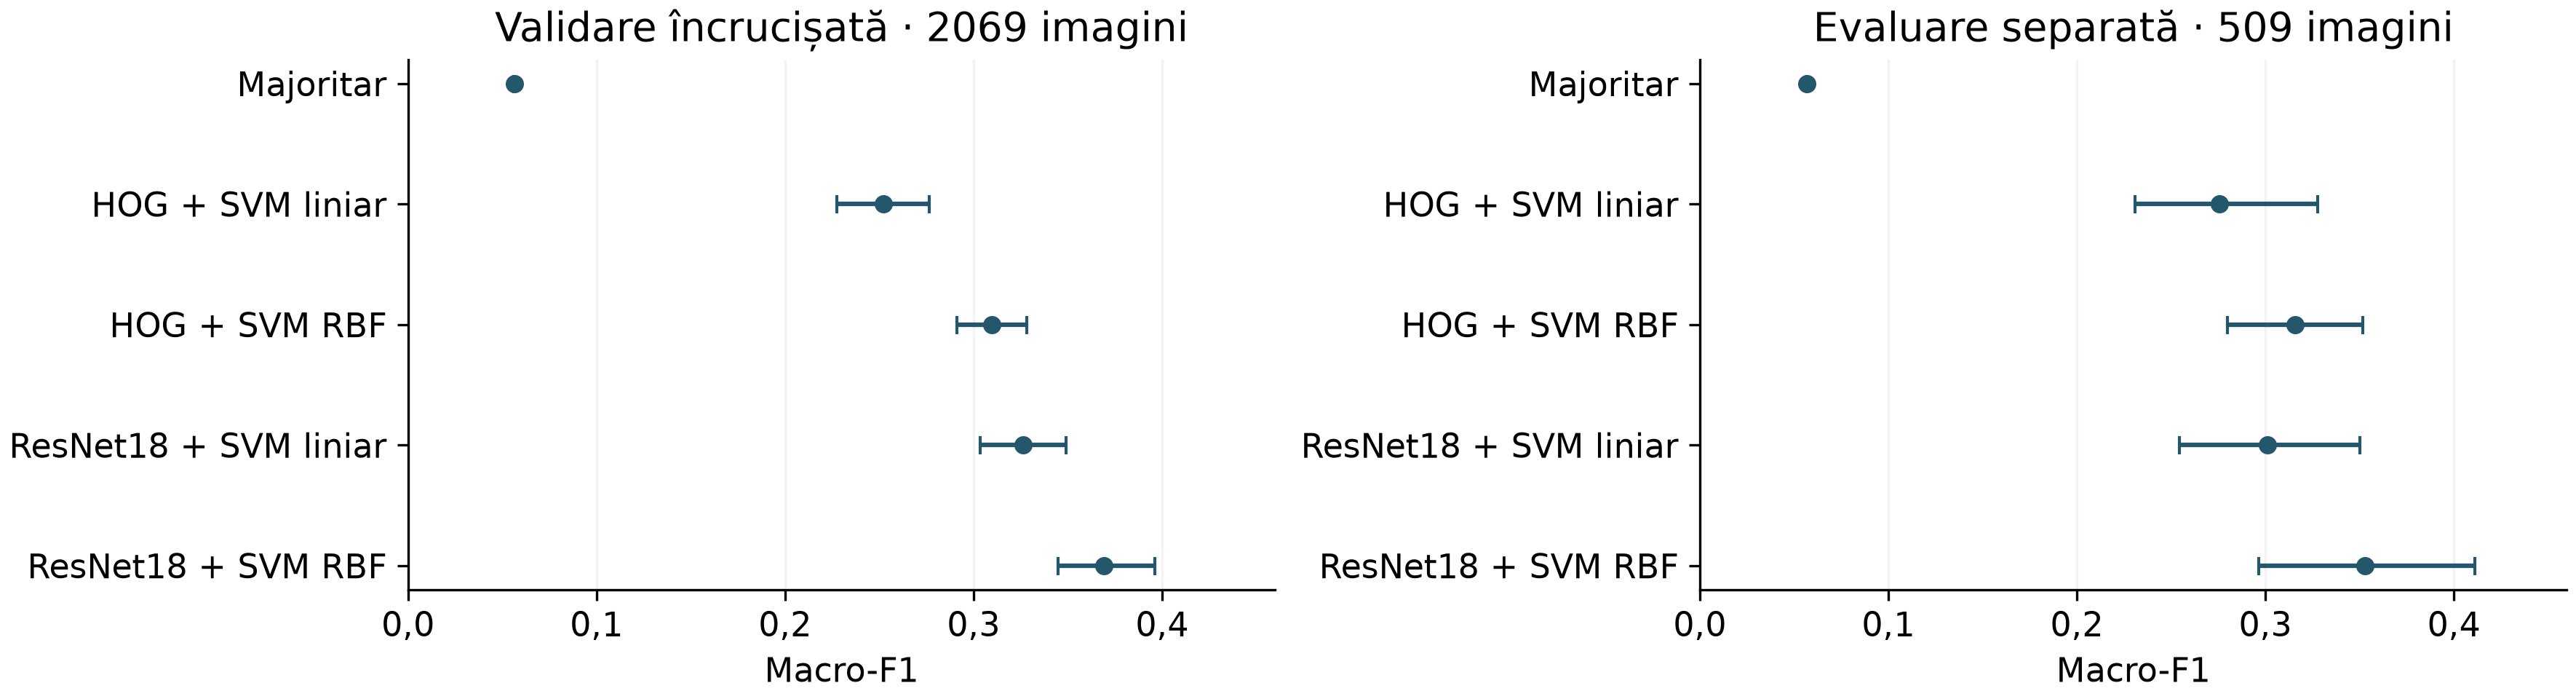
\includegraphics[width=\textwidth]{figuri/macro_f1_ro.png}
\caption{Macro-F1 și intervale bootstrap de 95\%, condiționate de predicțiile salvate. Punctul este scorul, iar segmentul este intervalul.}
\label{fig:macro}
\end{figure*}

\begin{figure*}[!t]
\centering
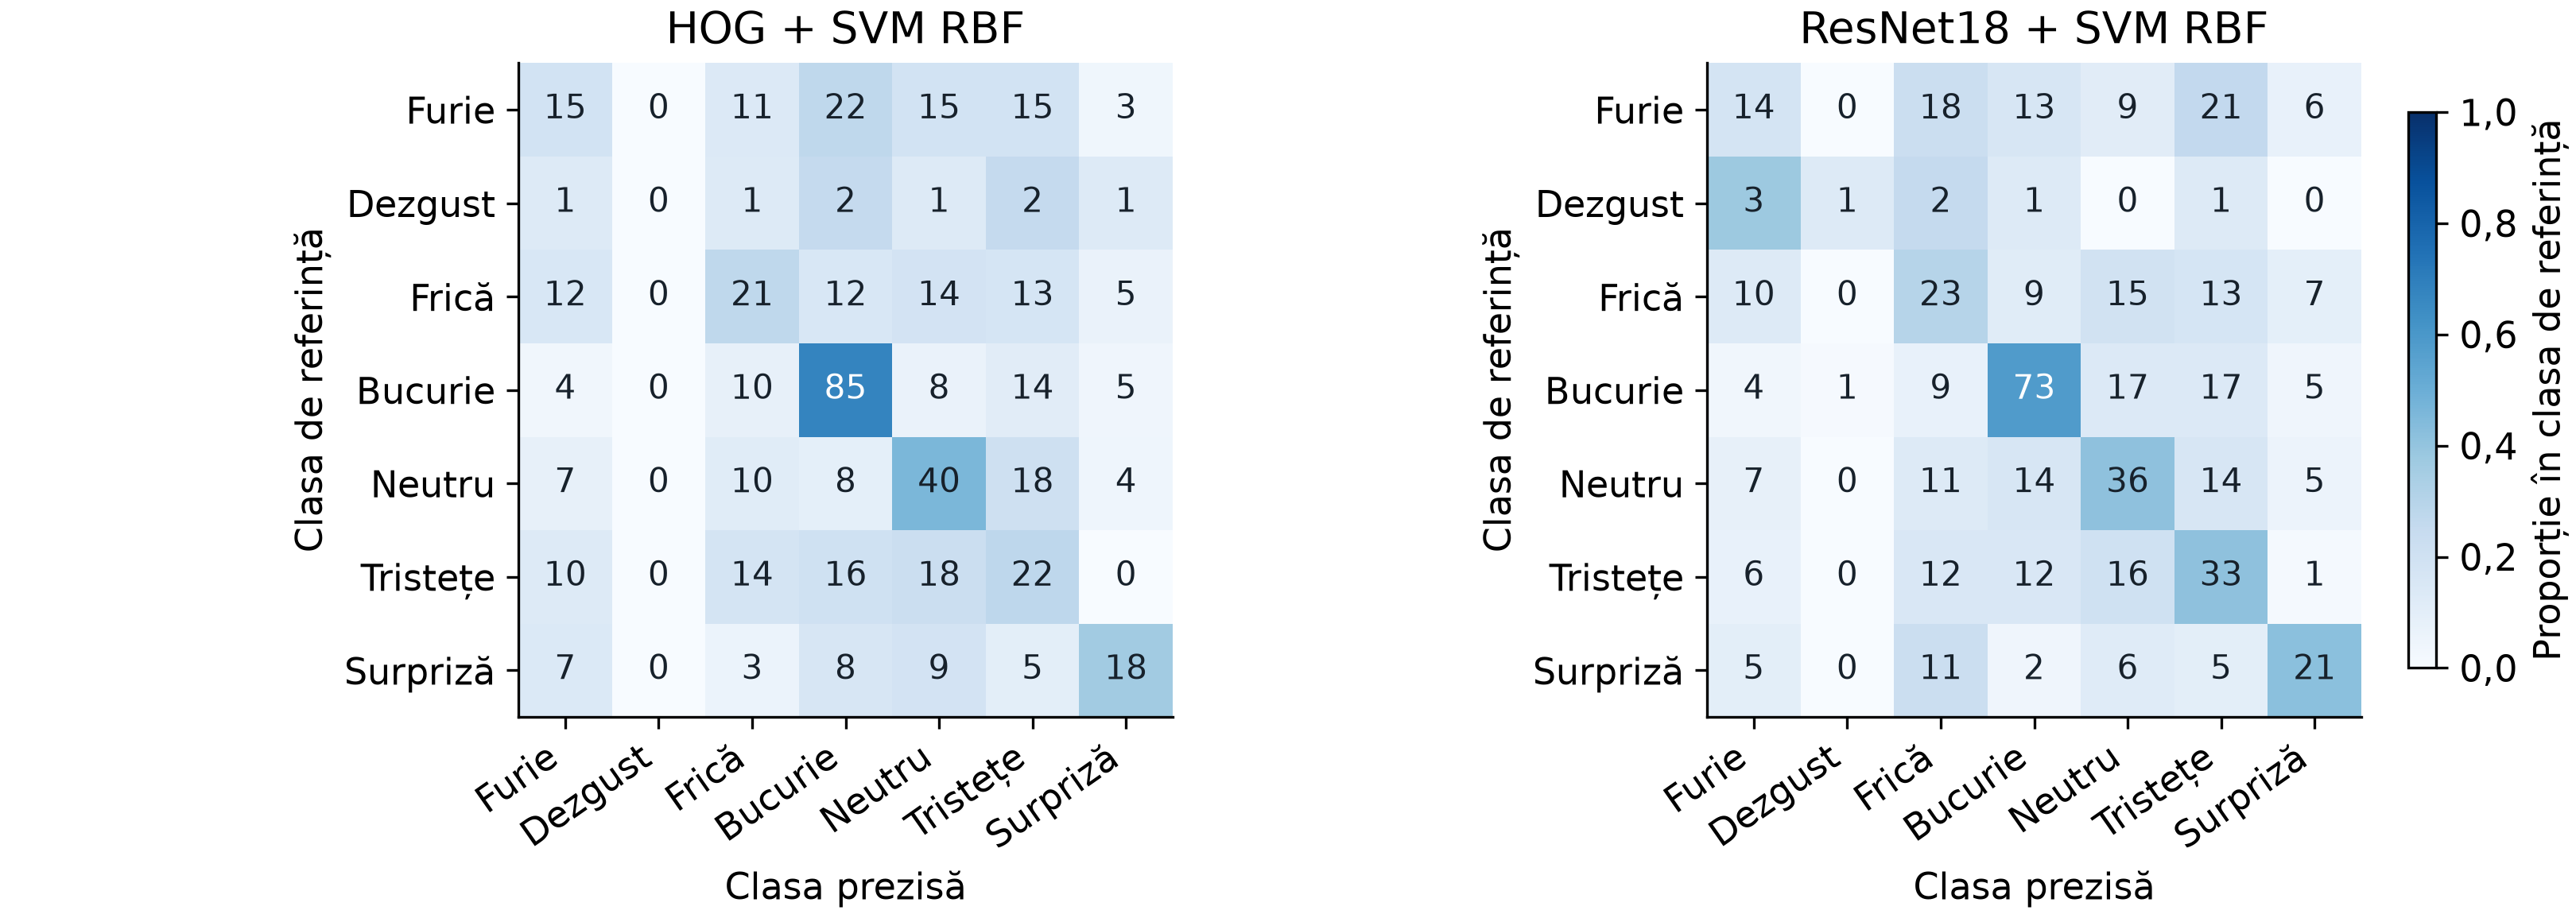
\includegraphics[width=0.92\textwidth]{figuri/confuzii_rbf_ro.png}
\caption{Cele două modele RBF pe setul separat. Numerele sunt imagini, iar culoarea arată proporția în fiecare clasă de referință. Matricele celorlalte două modele se află în exporturile numerice.}
\label{fig:confuzii}
\end{figure*}

\section{Rezultate comparative}
Tabelul~\ref{tab:scoruri} și Fig.~\ref{fig:macro} prezintă scorurile celor cinci modele pe aceleași imagini.

\begin{table}[!t]
\caption{Scoruri pe aceleași imagini pentru toate modelele: 2069 în validarea încrucișată și 509 în evaluarea separată}
\label{tab:scoruri}
\centering
\resizebox{\columnwidth}{!}{\begin{tabular}{lrrrr}
\toprule
& \multicolumn{2}{c}{Validare încrucișată} & \multicolumn{2}{c}{Evaluare separată} \\
\cmidrule(lr){2-3}\cmidrule(lr){4-5}
Model & Acuratețe (\%) & Macro-F1 & Acuratețe (\%) & Macro-F1 \\
\midrule
Majoritar & 24,55 & 0,0563 & 24,75 & 0,0567 \\
HOG + SVM liniar & 28,66 & 0,2520 & 30,84 & 0,2758 \\
HOG + SVM RBF & 39,29 & 0,3096 & 39,49 & 0,3157 \\
ResNet18 + SVM liniar & 37,60 & 0,3263 & 33,99 & 0,3011 \\
ResNet18 + SVM RBF & 44,03 & 0,3692 & 39,49 & 0,3528 \\
\bottomrule
\end{tabular}
}
\end{table}


\subsection{Reprezentarea și clasificatorul}
În validarea încrucișată, ResNet18 cu SVM RBF obține cel mai mare macro-F1 dintre configurațiile testate: 0,3692. HOG cu același tip de SVM obține 0,3096. Diferența este 0,0596, cu interval pereche de 95\% [0,0317; 0,0876], în sensul condiționat explicat în metodologie.

Alegerea clasificatorului contează pentru ambele reprezentări. Înlocuirea SVM liniar cu RBF crește macro-F1 de la 0,2520 la 0,3096 pentru HOG și de la 0,3263 la 0,3692 pentru ResNet18. Reprezentarea este astfel evaluată împreună cu tipul de SVM folosit. Parametrii selectați pe întreaga dezvoltare sunt $C=0,1$ pentru ambele variante liniare și $C=10$ pentru ambele variante RBF.

\subsection{Ce arată reperul majoritar}
Predictorul majoritar are 24,75\% acuratețe pe setul separat, dar numai 0,0567 macro-F1. El recunoaște exclusiv bucuria, cea mai frecventă clasă. Diferența dintre metrici arată de ce acuratețea singură este insuficientă pentru acest eșantion dezechilibrat.

\subsection{Aceeași acuratețe, erori diferite}
Pe cele 509 imagini separate, HOG-RBF și ResNet18-RBF clasifică fiecare corect 201 imagini, adică 39,49\% acuratețe. Macro-F1 este însă 0,3157 pentru HOG și 0,3528 pentru ResNet18, deoarece erorile sunt distribuite diferit între clase.

Diferența macro-F1 ResNet18 minus HOG este 0,0371. Intervalul pereche de 95\% este [$-$0,0235; 0,0972] și include zero. În acest eșantion, diferența observată nu susține o concluzie fermă de superioritate între variantele RBF.

\subsection{Costul calculului}
Rularea completă a durat 114,80 secunde, incluzând extragerea caracteristicilor, 240 de ajustări SVM, predicțiile și bootstrap-ul. Extragerea pe toate cele 2578 de imagini active a durat 0,95 secunde pentru HOG și 27,18 secunde pentru ResNet18.

Trăsăturile fixe sunt calculate o singură dată și reutilizate, iar scalerele sunt ajustate separat în fiecare antrenare. Măsurarea folosește un Intel Core i5-13600KF, fără CUDA și cu maximum patru fire Torch. Timpii descriu o rulare pe loturi, nu latența unei aplicații interactive.

\section{Analiza erorilor pe clase}
Fig.~\ref{fig:confuzii} prezintă matricele de confuzie ale celor două modele RBF, iar Tabelul~\ref{tab:recall} rata de recunoaștere pe clase pentru toate modelele.


\begin{table}[!t]
\caption{Rata de recunoaștere în procente și numărul de imagini din fiecare clasă}
\label{tab:recall}
\centering
\resizebox{\columnwidth}{!}{\begin{tabular}{lrrrrr}
\toprule
Clasă & Imagini & HOG liniar & HOG RBF & ResNet liniar & ResNet RBF \\
\midrule
Furie & 81 & 22,2 & 18,5 & 28,4 & 17,3 \\
Dezgust & 8 & 12,5 & 0,0 & 12,5 & 12,5 \\
Frică & 77 & 33,8 & 27,3 & 33,8 & 29,9 \\
Bucurie & 126 & 42,9 & 67,5 & 47,6 & 57,9 \\
Neutru & 87 & 32,2 & 46,0 & 35,6 & 41,4 \\
Tristețe & 80 & 21,2 & 27,5 & 21,2 & 41,2 \\
Surpriză & 50 & 26,0 & 36,0 & 30,0 & 42,0 \\
\bottomrule
\end{tabular}
}
\end{table}

\subsection{Citirea confuziilor}
ResNet18-RBF recunoaște 33 dintre cele 80 de imagini de tristețe, față de 22 pentru HOG-RBF. Pe bucurie, ordinea se inversează: 73 dintre 126, față de 85. Câștigul nu este uniform pe clase.

Dezgustul are numai opt imagini. HOG-RBF nu recunoaște niciuna, iar ResNet18-RBF recunoaște una. Fiecare imagine schimbă rata cu 12,5 puncte procentuale, deci procentul trebuie citit împreună cu acest suport mic.

\section{Concluzii}
Studiul urmărește comparația de la imaginea verificată până la predicție și metrică. Controlul clasificatorului schimbă interpretarea comparației HOG--ResNet18, iar analiza pe clase explică de ce aceeași acuratețe poate ascunde scoruri macro-F1 diferite.

Manifestele, predicțiile și instrucțiunile sunt disponibile în repository-ul proiectului~\cite{own_repo}. Comanda \texttt{python scripts/verify\_published\_results.py} verifică integritatea exporturilor și recalculează metricile fără imagini sau ponderi. Refacerea antrenării necesită imaginile și ponderile verificate. Figurile și tabelele provin din rezultatele salvate.

\begin{thebibliography}{9}
\bibitem{fer} I. J. Goodfellow \emph{et al.}, ``Challenges in representation learning: A report on three machine learning contests,'' în \emph{Proc. ICONIP}, 2013. [Online]. Disponibil: \url{https://arxiv.org/abs/1307.0414}
\bibitem{hog} N. Dalal și B. Triggs, ``Histograms of oriented gradients for human detection,'' în \emph{Proc. CVPR}, 2005, pp. 886--893.
\bibitem{resnet} K. He, X. Zhang, S. Ren și J. Sun, ``Deep residual learning for image recognition,'' în \emph{Proc. CVPR}, 2016, pp. 770--778.
\bibitem{kaggle} M. Sambare, ``FER-2013,'' set de date Kaggle, versiunea 1. [Online]. Disponibil: \url{https://www.kaggle.com/datasets/msambare/fer2013}
\bibitem{duplicates} B. Barz și J. Denzler, ``Do we train on test data? Purging CIFAR of near-duplicates,'' \emph{Journal of Imaging}, vol. 6, nr. 6, art. 41, 2020, doi: 10.3390/jimaging6060041.
\bibitem{cv} Y. Bengio și Y. Grandvalet, ``No unbiased estimator of the variance of K-fold cross-validation,'' \emph{Journal of Machine Learning Research}, vol. 5, pp. 1089--1105, 2004.
\bibitem{barrett} L. F. Barrett \emph{et al.}, ``Emotional expressions reconsidered: Challenges to inferring emotion from human facial movements,'' \emph{Psychological Science in the Public Interest}, vol. 20, nr. 1, pp. 1--68, 2019, doi: 10.1177/1529100619832930.
\bibitem{license} Open Data Commons, ``Open Database License (ODbL) v1.0'' și ``Database Contents License (DbCL) v1.0.'' [Online]. Disponibil: \url{https://opendatacommons.org/licenses/}
\bibitem{own_repo} C.-A. Colăcel, ``Real-Time Emotion Recognition Platform,'' software. [Online]. Disponibil: \url{https://github.com/colacbrr/Real-Time-Emotion-Recognition-Platform}
\end{thebibliography}
\end{document}
